\section{Introduction}

Sparsest cut is a central problem among various graph partitioning tasks. Given a graph $G=(V,E, c)$, where $c\colon E \to \mathbb{N}$ is a capacity function, the goal is to find a subset of vertices $S\subseteq V$ that minimizes

\[
\phi\br{S} = \frac{c\br{S, \bar{S}}}{\spr{S}\cdot \spr{\bar{S}}}.
\]
where $\bar{S}=V\setminus S$ and $c\br{S,\bar{S}}=\sum_{u\in S}\sum_{v \in \bar{S}}c\br{u, v}$.

This problem has been extensively studied in the literature resulting in remarkable connections to topics including metric spaces and spectral graph theory with the state-of-the-art approximation algorithm due to Arora, Rao, and Vazirani \cite{ExpanderFlowsGeometricEmbeddingsAndGraphPartitioning}, achieving an approximation ratio of $\bigo\br{\sqrt{\log n}}$, where $n=\spr{V}$. Moreover, it also has a number of applications as an essential primitive in other graph algorithms, where it serves as a building block for various divide-and-conquer strategies. This includes graph partitioning where the goal is to find a subset of edges of minimum capacity such that all of the connected components resulting from deleting these edges are of small size. Another example is the problem of hierarchical clustering with similarity measures, where the goal is to hierarchically cluster data points, so that to minimize the Dasgupta's clustering objective. Intuitively, this objective promotes clusters with both children of balanced size as well as a low capacity of edges cut between them. In particular, given an $\alpha$-approximation algorithm for the sparsest cut, one can obtain an $\bigo\br{\alpha}$-approximation algorithm for both of the aforementioned problems \cite{ExpanderFlowsGeometricEmbeddingsAndGraphPartitioning,HierarchicalClusteringObjectiveFunctionsAndAlgorithms,ApproximateHierarchicalClusteringViaSparsestCutAndSpreadingMetrics}.

This usefulness of sparsest cut can be attributed to the following observation, implicitly exploited by many algorithms.
The quantity $\spr{S}\cdot \spr{\bar{S}}$ can be interpreted in two separate ways. First, imagine each pair of vertices to be associated with a unit demand. Then, $\spr{S}\cdot \spr{\bar{S}}$ can be seen as the total demand crossing the cut. This interpretation is useful for the sake of developing approximation algorithms for the sparsest cut itself, since a weak duality between sparsest cut and multicommodity flow type problems has been established \DD{[tutaj by sie przydalo cytowanie, jesli mozliwe]}. Secondly, $\spr{S}\cdot \spr{\bar{S}}$ can be observed to be large when both partitions are of roughly equal size. This comes useful when developing divide and conquer algorithms for other graph problems, since the product in the denominator becomes a measure of the balance of a cut.

However, if one were to generalize the sparsest-cut to general demands setting, these two interpretations are no longer equivalent. Let $w\colon V\times V\to \mathbb{N}$ be a demand function.
The \emph{generalized sparsest cut problem} \DD{usunalem ``with demands'' gdyz dalej tak bylo} is to find a subset of vertices $S\subseteq V$ that minimizes
\[\phi_w\br{S} = \frac{c\br{S, \bar{S}}}{w\br{S, \bar{S}}}.
\]
This problem is also well-understood, and the state-of-the-art approximation algorithm is due to Arora, Lee, and Naor \cite{EuclideanDistortionAndTheSparsestCut}, which achieves the ratio of $\bigo\br{\sqrt{\log n}\cdot \log \log n}$. However, as discussed above, in order to use the some notion related to sparsity in a wider range of applications, it would be desirable to approximate some quantity measuring the balance of a cut. 
To the best of our knowledge, no such results have been obtained in the literature yet.
The graph \emph{conductance} is a well-known measure of the balance of a cut, defined as
\[
\phi\br{S} = \frac{c\br{S, \bar{S}}}{\operatorname{vol}(S)\cdot \operatorname{vol}(\bar{S})}.
\]
where $\operatorname{vol}(S)=\spr{\brc{e\in E\colon e\cap S\neq \emptyset}}$\footnote{Note, that there are several similar definitions of the conductance, however they are all equivalent up to constant factors.}. In fact, for the case of unit demands, the conductance is equivalent to the sparsest cut, up to a constant factor. However, for the general demands this is not a case, and this will come useful in our applications. The \emph{generalized conductance} of a cut $\br{S,\bar{S}}$ will be, defined as
\[
\psi_w\br{S} = \frac{c\br{S, \bar{S}}}{w\br{S, V}\cdot w\br{\bar{S}, V}}.
\]
The problem of $\psi_w$ minimization will be called the \emph{minimum generalized conductance} problem.
\DD{tutaj usunalem powtorzenie, ze to nie bylo studiowane (zwlaszcza, ze piszemy, ``we introduce ...'' powyzej}
%To the best of our knowledge, this objective has not been studied in the literature yet, and it is not known whether it admits an algorithm with a non-trivial approximation ratio.
We initiate the study of this problem by providing an $\bigo\br{\log n}$-approximation algorithm for general graphs.
Interestingely enough, in our algorithm we use a non-trivial reduction to the former generalized sparsest cut with demands, i.e., the minimization of $\phi_w$.
\DD{dalej uproscilem, gdyz bez definicji robi sie to za malo formalne chyba. A za chwile i tak wszystko bedzie w ``our results''.}
%However, in order for the approximation ratio to be preserved, \DD{powyzsze nie wskazuje, ze ``zachowujemy'' app. ratio, a raczej dostajemy nieco gorsze} additional constraint expressing the maximum amount of demand cut is required. We call this problem a constrained sparsest cut problem and show, how to solve it using
At the core of our method are algorithmic reductions to few cut-like problem, including the one just mentioned as an example, and the notion of
cut-sparsifier tree decompositions by R\"{a}cke \cite{OptimalHierarchicalDecompositionsForCongestionMinimizationInNetworks}.
%Since the embedding \DD{piszac ``the'' embedding odnosimy sie do kontekstu, ale nie jest jasne jaki embedding mamy na mysli.} step incurses an $\bigo\br{\log n}$ distortion and one can the constrained sparsest cut on trees in polynomial time, we get the desired approximation ratio.

%It should be noted, that this is not the only possible balance-oriented generalization of the sparsest cut. For instance, one could also consider the following ratio:
% \[
% \psi'_w\br{S} = \frac{c\br{S, \bar{S}}}{w\br{S}\cdot w\br{\bar{S}}}.
% \]
%However, the first objective $\psi_w\br{S}$ is more natural due to the fact that it also takes into account the demands crossing the cut, since $w\br{S, V}= w\br{S}+w\br{S, \bar{S}}$. As it turns out, this becomes crucial for the applications we have in mind, and thus we focus on $\psi_w\br{S}$.
\DD{mam mieszane odczucia, czy ta koncowka wiecej nie namiesza niz pomoze. Otwiera bowiem watpliwosc czy nie jest sytuacja taka, ze studiuje sie wybrany sobie jeden wariant z wielu i recenzent sie zacznie zastanawiac dlaczego ten jest lepszy niz inny. Trzymalbym sie zatem narracji: po pierwsze uogolnienie, wiec dobrze, po drugie problem nietrywialny, wiec dobrze; po trzecie jest naturalna interpretacja; po czwarte uzyteczny. Tu by byla kropka. Chodzi o to, ze ludzie czesto sa oporni do prac wprowadzajacych nowy problem, gdyz sa cale morza prac, ktore to czynia i wiekszosc tych podproblemow i wariantow zwyczajnie nie jest zbyt ciekawa (lub interasujaca dla waskiego grona). Na razie zakomentowalem.
Moze do podsumowania taka dyskusja?}

\subsection{Our results and techniques}

\DD{todo: na razie zosstawilem;}
In this work, we show a series of algorithmic reductions between a large number of problems. The generalized conductances turns out to be the central one of them. Due to this we structure our work into two main parts.

Firstly, we concern ourselves with approximating the latter problem. To do so, we combine a variety of techniques in order to simplify the problem. Intuitively, our algorithm is sensitive to two types of instances which are tackled differentily. Although our algorithm never distinguishes between them explicitly, by choosing the best among two obtained solutions we get a non-trivial approximation ratio of $\bigo\br{\log n}$. The two cases are dictated by the size of $w\br{S, \bar{S}}$. If this quantity is large enough, then the problem (up to a constant factor approximation loss) essentially becomes the well known $k$-multicut problem, where the task is to minimize the cost of cut edges while ensuring that at least $k$ unit of demands are partitioned. The only difference is that here the number of connected components outputed by the algorithm might be arbitrarily large. To remedy this we employ a max-cut algorithm which ensures that a significant portion of the demand is still cut while partitioning the components into two groups as required.

If the aforementioned quantity is small, then we show that we can reduce the problem to the classic sparsest-cut with additional constraint that the demand cut cannot be too large. This is done by constructing an auxiliary graph with new demand function such that cutting demand in this new instance roughly corresponds to minimizing the conductance in the original instance. This reduction preserves the approximation ratio, however its analysis is sensitive and crucially relies on the fact that $w\br{S, \bar{S}}$ is assumed to be of small value. 

In order to tackle this constrained version of the sparsest cut we use a general technique by \cite{OptimalHierarchicalDecompositionsForCongestionMinimizationInNetworks}. The idea is to embed a graph into a polynomial-sized convex combination of trees, which in expectance preserves the value of any cut up to $\bigo\br{\log n}$ distortion. This allows us to obtain the $\bigo\br{\log n}$-approximation by solving the problem to optimality on all trees and outputting the best of the solutions. This indeed becomes an easy task, since the (unconstrained) sparsest cut can be found in a tree by only considering cuts with singular edge cut. As it turns out, the same is true for the constrained version of the problem.

\DD{todo: tutaj skleic...} This problem admits an $\beta=\bigo\br{\log n}$-approximation algorithm by combining \cite{AUnifiedApproachToApproximatingPartialCoveringProblems} with \cite{OptimalHierarchicalDecompositionsForCongestionMinimizationInNetworks}.
\DD{to by moze poszlo do frontu do our results:}
\begin{corollary}
  There is a polynomial-time $O(\log n)$-approximation algorithm for the problem of minimizing $\psi_w\br{G}$ on general graphs as well as an $O(1)$-approximation algorithm for the problem of minimizing $\psi_w\br{G}$ on trees.
\end{corollary}

In the second part of the paper we move ourselves towards applications of the generalized conductance. We show that by iterative application of the above algorithm we can partition the graph into components with demand at most $\frac{4}{5}\cdot w\br{V}$ while paying only $\bigo\br{\log n}$ times more than it is required to partition the graph into components with demand at most $w\br{V}/2$. Therefore, the algorithm is a bicriteria approximation.
% It should be noted, that there is an evidence that no true polylogarithmic approximation for this task exists [cite here].

Then, we show that the above bicriteria approximation algorithm can be used to obtain an $\bigo\br{\log n}$-approximation for hierarchical clustering with demands. This is done in a recursive top-down manner. The algorithm starts by finding a graph partition consisting of components with demand at most $\frac{4}{5}\cdot w\br{V}$. Then, the rest of hierarchy is build by applying the algorithm recursively in all of the resulting clusters. Using a tight analysis generalizing the framework of \cite{ApproximateHierarchicalClusteringViaSparsestCutAndSpreadingMetrics} we show that the approximation ratio is indeed preserved.

Figure \ref{fig:reductions} shows the algorithmic reductions that appear in this work.

\begin{figure}[H]
  \centering
  \resizebox{\textwidth}{!}{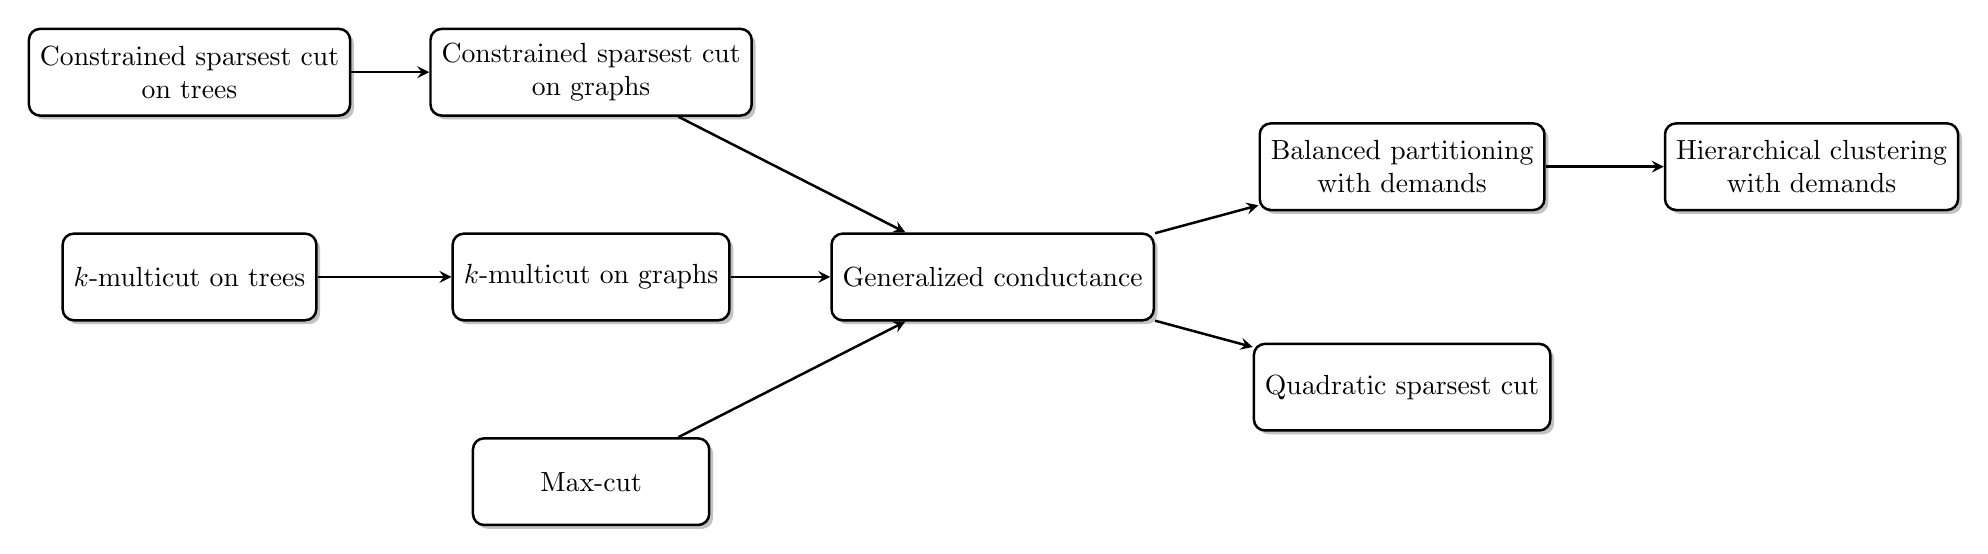
\begin{tikzpicture}[>=stealth, line width=0.9pt]
  \tikzstyle{box}=[draw, rounded corners, align=center, inner sep=4pt,
    minimum width=3cm, minimum height=1.10cm,
    fill=white,
    preaction={fill=black,opacity=0.24,transform canvas={xshift=1.4pt,yshift=-1.4pt}}]

  % Left: tree problems
  \node[box] (cst) at (0, 2.6) {Constrained sparsest cut\\on trees};
  \node[box] (kmt) at (0, 0.0) {$k$-multicut on trees};

  % Middle-left: graph problems + max-cut
  \node[box] (csg) at (5.1, 2.6) {Constrained sparsest cut\\on graphs};
  \node[box] (kmg) at (5.1, 0.0) {$k$-multicut on graphs};
  \node[box] (mc)  at (5.1, -2.6) {Max-cut};

  % Center: target problem
  \node[box, minimum width=3cm] (gc) at (10.2, 0.0) {Generalized conductance};

  % Right: applications
  \node[box] (bpd) at (15.4, 1.4) {Balanced partitioning\\with demands};
  \node[box] (qsc) at (15.4, -1.4) {Quadratic sparsest cut};
  \node[box] (hcd) at (20.6, 1.4) {Hierarchical clustering\\with demands};

  \draw[->] (cst) -- (csg);
  \draw[->] (kmt) -- (kmg);

  \draw[->] (csg) -- (gc);
  \draw[->] (kmg) -- (gc);
  \draw[->] (mc)  -- (gc);

  \draw[->] (gc) -- (bpd);
  \draw[->] (gc) -- (qsc);
  \draw[->] (bpd) -- (hcd);
\end{tikzpicture}
}
  \caption{Reduction map of problems and applications considered in this paper.}
  \label{fig:reductions}
\end{figure}
\subsection{Related work}

